\chapter{Ergebnisse}
Aufgrund der Architektur des CTA´s bietet sich eine Mittelwertbildung über die Teleskope, die das gleiche Schauer gesehen
haben, an, um die Performance des Schätzers zu verbessern.
Zusätzlich scheint aufgrund der Tatsache, dass die Energie des primär Teilchens proportional zur Schauergröße ist und das
ganze Array eine bessere Aussage über die Größe treffen kann als einzelne Teleskope, eine Zusammenfassung der
Information aller Teleskope sinnvoll.
Da das in \autoref{sec:RF} beschriebene Kriterium sich auf den absoluten Fehler und nicht auf den relativen Fehler
bezieht, muss der Tatsache, dass die richtige Schätzung großer Energien für den Algorithmus einen größeren Gewinn bedeutet,
durch Transformationen entgegengesteuert werden, um eine gute Energieauflösung in allen Energiebereichen zu erlangen.

\section{Energie Rekonstruktion mit Hilfe eines Random Forest Regressors}
\label{sec:first}

Um ein Vergleichsergebnis zu erhalten, wird zunächst ein RandomForest Regressor, wie er in \autoref{sec:RF} beschrieben wird, verwendet,
der eine Energieschätzung für jedes Teleskop vornimmt.
Für das Training werden nur Gamma Ereignisse verwendet und somit eine erfolgreiche Signal-Untergrund Trennung vorrausgesetzt.
Für ein realitätstreueres Testen werden zerstreute und punktgerichtete Gamma Simulationsdaten verwendet, da in der
Realität die Signal Extraktion nicht zwischen punktgerichteten Photonen und Photonen, die in der Atmosphäre entstehen oder zu der
allgemeinen kosmische Strahlung gehören, unterscheiden kann.

Als Attribute werden die nicht richtungsabhängigen Hillasparameter verwendet, dazu gehören Intensität, Länge, Weite, Schiefe und Wölbung, sowie
die totale Intensität, die von allen Teleskopen aufgenommen wird.
Zusätzlich werden die Anzahl der ausgelösten Teleskope, SST, MST und LST als Attribute genutzt, sowie die Identifikationsnummer des
Teleskopes, welche für das LST $1$, für das MST $2$ und für das SST $3$ ist.

Desweiteren werden die skalierte Länge
\begin{equation}
  SW = \frac{w- \langle w \rangle}{\sigma_w}
\end{equation}
und Weite
\begin{equation}
  SL = \frac{l - \langle l \rangle}{\sigma_l}
\end{equation}
verwendet, wobei der Mittelwert über alle Trainingsdatenwerte genommen wird. Diese Methode nennt sich Scaled Cuts Technik.\cite[104]{HESS}

Der ganze Datensatz besteht aus $\num{3322938}$ Datenpunkten, die in $\SI{33}{\percent}$ Trainings- und $\SI{66}{\percent}$ Testdatensatz aufgeteilt werden.
Die Aufteilung geschieht jedoch mithilfe der Ereignisnummer, damit bei der Trennung keine Ereignisse getrennt werden.

Bei dem Training wird ein Random Forest verwendet, der zur Verhinderung des Übertrainings eine Maximal Tiefe von $10$ Ebenen besitzt.
Jeder Baum trainiert mit $\sqrt{N}$ Attributen, wobei $N$ Attribute zur Verfügung stehen, um Korreliertheit der Bäume zu vermeiden,
was zu gleichen Baumstrukturen führen würde und somit zu bevorzugten Ergebnissen.
Außerdem besteht der Wald aus $100$ Bäumen, was mit einer größeren Rechenleistung vergrößert werden kann, ohne
das es, wie in \autoref{sec:RF} erklärt, zum Übertraining kommt.
Der Algorithmus nutzt das in \autoref{sec:RF} beschriebene Kriterium der Varianz Reduktion und da die gering gewählte Tiefe
ein Übertraining bereits verhindert und das Problem viel Statistik besitzt, werden die Hyperparameter
der minimalen Blatt und Trenngröße auf ihrer Grundeinstellung von $1$ und $2$ gelassen.

\begin{figure}
  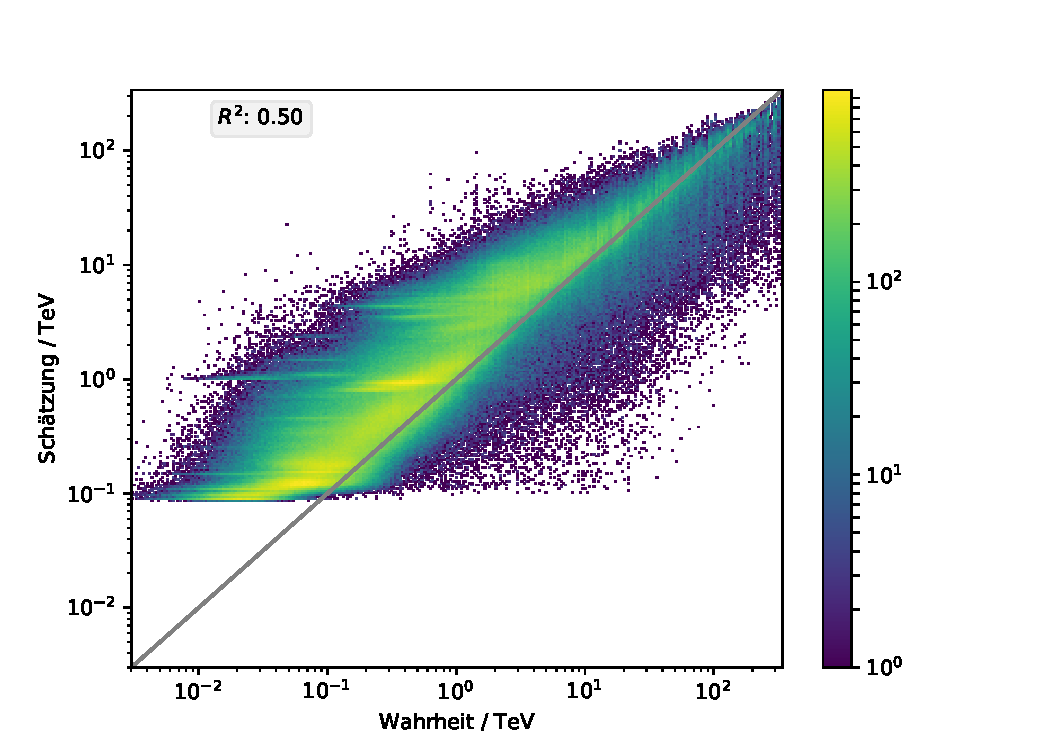
\includegraphics[width=0.7\textwidth]{Plots/RF.pdf}
  \centering
  \caption{In diesem Graph ist die vorhergesagte Energie gegen die Wahrheit aufgetragen, wobei Streuung und Verzerrung um die
          Diagonale zu erkennen sind.}
  \label{abb:Energie_RF}
\end{figure}
Dieser trainierte Entscheidungswald wird mit $\num{2193140}$ Datenpunkten getestet und liefert eine Performance, wie sie in \autoref{abb:Energie_RF} zu sehen ist.
Dabei ist eine Überschätzung der Wahrheiten zu beobachten sowie feine horizontale Linien, die auf eine Korreliertheit der Entscheidungsbäume hindeuten.
Der $R^2$-Wert von $\num{0.50}$ deutet auf eine bessere Beschreibung des Modells als der bloße Mittelwert hin.
Die Korreliertheit und die Verzerrung kann durch eine geeignetere Wahl der Hyperparameter minimiert werden, jedoch ist dies nicht Ziel dieser
Arbeit.

\begin{figure}
  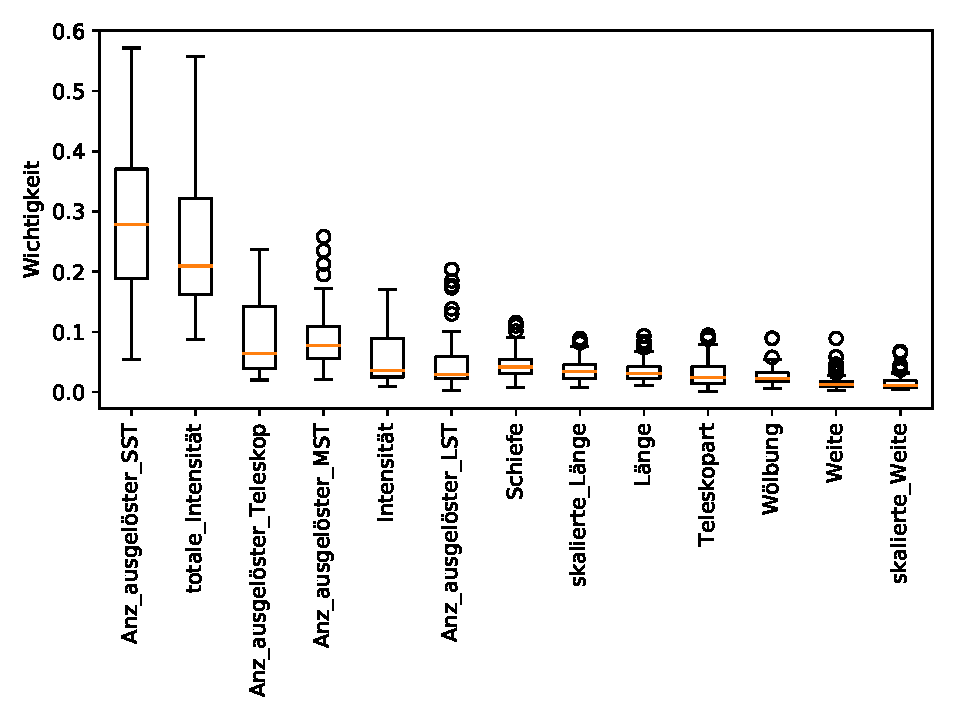
\includegraphics[width=0.7\textwidth]{Plots/feautureimportance_boxplot_firstForest.pdf}
  \centering
  \caption{Darstellung der Wichtigkeit der genutzen Attribute bei der ersten Vorhersage als Kastengrafik. Die Anzahl der ausgelösten SST und die totale Intensität
          stellen die wichtigsten Attribute dar und die Weite der Hillasellipse trägt kaum zur Schätzung bei.}
  \label{abb:first_FI}
\end{figure}
Wie in \autoref{abb:first_FI} dargestellt, besitzen eventspezifische Attribute wie die Anzahl der ausgelösten Teleskope und die totale Intensität die größte Wichtigkeit und teleskopspezifische Attribute
wie die Hillasparameter liefern keinen großen Informationsgewinn.
Eine Erklärung liefert die Tatsache, dass die in dem Schauer deponierte Energie ein wichter Parameter für die Energieschätzung ist und die Hillasparameter im
Gegensatz zu den eventspezifischen Parametern von dem Abstand des Teleskopes zum Schauer abhängen.
Aufgrund der Unterschiedlichkeit der Attribute kann die Wichtigkeit nach \autoref{sec:Per} eine Verzerrung besitzen und Attribute
wie die Intensität überschätzt, sowie Attribute wie die Teleskopart unterschätzt werden.

\section{Optimierung durch Mittelwerte und geeignete Gewichte}

Die Energieschätzung der einzelnen Teleskope bei einem Ereignis variiert, obwohl sie das gleiche Schauer beobachten.
Dies liegt an dem unterschiedlichen Blickwinkel und Abstand der Teleskope, was dazu führt das jedes Teleskop unterschiedlich viel Information über das
Schauer besitzt.
Wenn die variierenden Ergebnisse zufällig und nach dem Zentralen Grenzwertsatz der Statistik normalverteilt um den
wahren Wert liegen\cite[10]{zufall_Fehler}, verbessert eine Mittelwertbildung das Ergebnis.
Daher wird als Schätzer das arithmetische Mittel und der Median untersucht.
\begin{figure}
  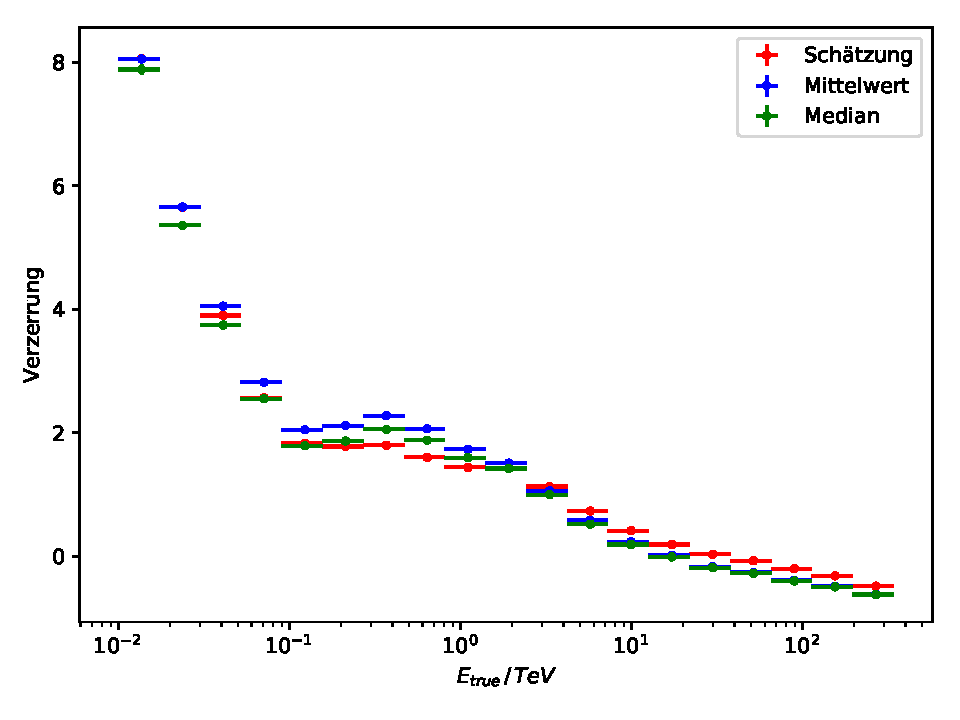
\includegraphics[width=0.7\textwidth]{Plots/RF_mean_bias.pdf}
  \centering
  \caption{Darstellung der Verzerrung für verschiedene Energiebereiche. Es sind die Mittelwerte der relativen Fehler für die erste Vorhersage, die Vorhersage
          nach der Mittelwertbildung und der Median der Vorhersagen aufgetragen.}
  \label{abb:mean_median_bias}
\end{figure}
\begin{figure}
  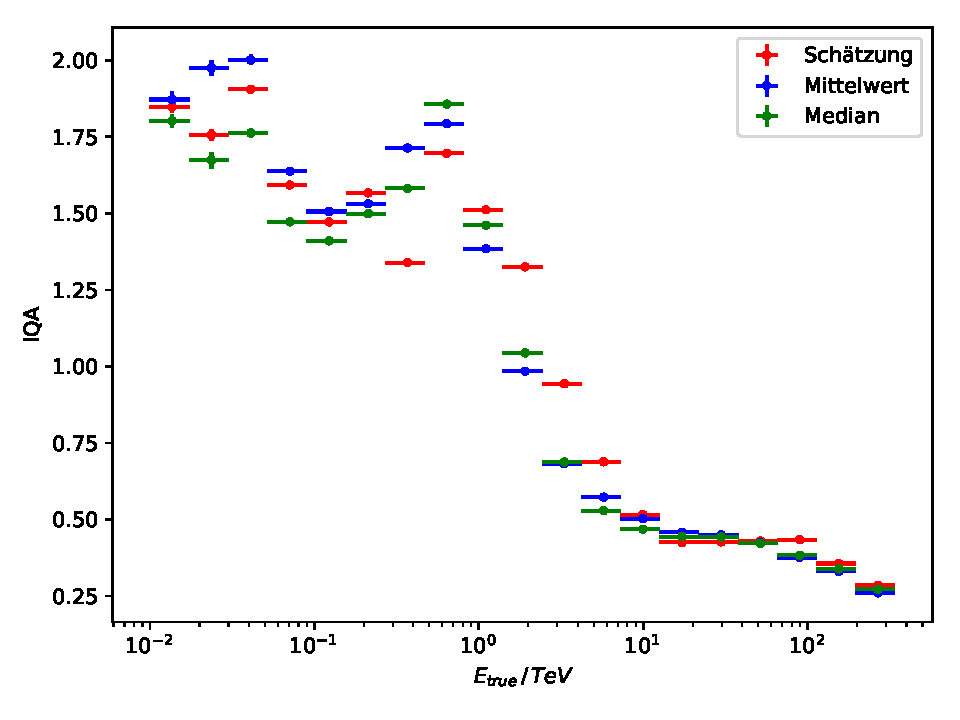
\includegraphics[width=0.7\textwidth]{Plots/RF_mean_resolution.pdf}
  \centering
  \caption{Darstellung des IQA des relativen Fehlers für verschiedene Energiebereiche. Aufgetragen sind die erste Vorhersage, die Vorhersage
          nach der Mittelwert Bildung und der Median der Vorhersagen.}
  \label{abb:mean_median_IQA}
\end{figure}

Die zusammengefassten Schätzungen führen auf die Verzerrungen und IQA's, die in \autoref{abb:mean_median_bias} und \autoref{abb:mean_median_IQA} zusehen sind.
Bei geringen Energien führt das arithmetische Mittel auf keine geringere Verzerrung und auch der Median bringt nur eine leichte Verbesserung.
Dies liegt daran, dass eine Verzerrung die Annahme verletzt, dass die Ergebnisse um den wahren Wert liegen, stattdessen liegen sie um einen verschobenen
Wert.
Das arithmetische Mittel kann eine Verzerrung nicht verringern.
Nur bei Ereignissen mit einer geringen Verzerrung sorgt das Mitteln für eine bessere Performance, was zum einen bei dem IQA für große Energien zu beobachten
ist und bei dem gemittelten quadratischen Fehler, der von $\SI{103.31}{\tera\eV\squared}$ für die erste Schätzung auf $\SI{66.69}{\tera\eV\squared}$ nach einer
Mittelwertbildung fällt.

Das der Median die Verzerrung verringert liegt daran, dass es bei dem Beobachten von Schauern vorkommen kann, dass einzelne Teleskope im Gegensatz zu anderen
besser positionierten Teleskopen nur einen geringen Teil des Schauers beobachten und somit weniger Information des Schauers besitzen, was zu einer falsche Vorhersage
führt.
Da dies meist nur auf vereinzelte Teleskope zutrifft, liegt der Median der Teleskope richtig.
Dies zeichnet sich auch durch einen gemittelten quadratischen Fehler von $\SI{68.11}{\tera\eV\squared}$ aus, welcher besser als der Fehler der ersten Schätzung ist und
vergleichbar mit dem Fehler der Mittelwertbildung.

Eine weitere Möglichkeit um das Problem, dass nicht alle Telskope das Schauer gleich gut sehen, zu beheben, stellt das Mitteln mit einem Gewicht, welches die
Sichtbarkeit des Schauers beschreibt, dar.
Ein Indiz auf den gesehenen Anteil des Schauers stellt die beobachtete Intensität dar , wobei eine hohe
Intensität eine gute Sichtbarkeit bedeutet und somit die Intensität direkt als Gewicht verwendet wird.

Zum Anderen besitzten die in \autoref{sec:CTA} beschriebenen Teleskope eine energieabhängige Sensitivität, wobei
es einen Energiebereich gibt, indem eine volle Sensitivität herrscht und einen indem eine Teilsensitivität
herrscht.
Das LST besitzt eine Teilsensitivität bei $\SI{20}{\giga\eV}-\SI{3}{\tera\eV}$ und eine volle Sensitivität bei
$\SI{20}{\giga\eV}-\SI{150}{\giga\eV}$.
Das MST ist teilsensitiv bei $\SI{80}{\giga\eV}-\SI{50}{\tera\eV}$ und vollsensitiv bei $\SI{150}{\giga\eV}-\SI{5}{\tera\eV}$
und das LST hat seinen Teilsensitivitätsbereich bei Energien zwischen $\SI{1}{\tera\eV}-\SI{300}{\tera\eV}$ und seine
Hauptsensitivität bei $\SI{5}{\tera\eV}-\SI{300}{\tera\eV}$.\cite{CTA_tec}
Wenn die geschätzte Energie im vollsensitiven Bereich liegt, wird ein Gewicht von $2$ angelegt, wenn sie im
teilsensitiven Bereich liegt ein Gewicht von $1$ und wenn die Energie in keinem Sensitivitätsbereich liegt,
wird ein Gewicht von $0.1$ angelegt.
\begin{figure}
  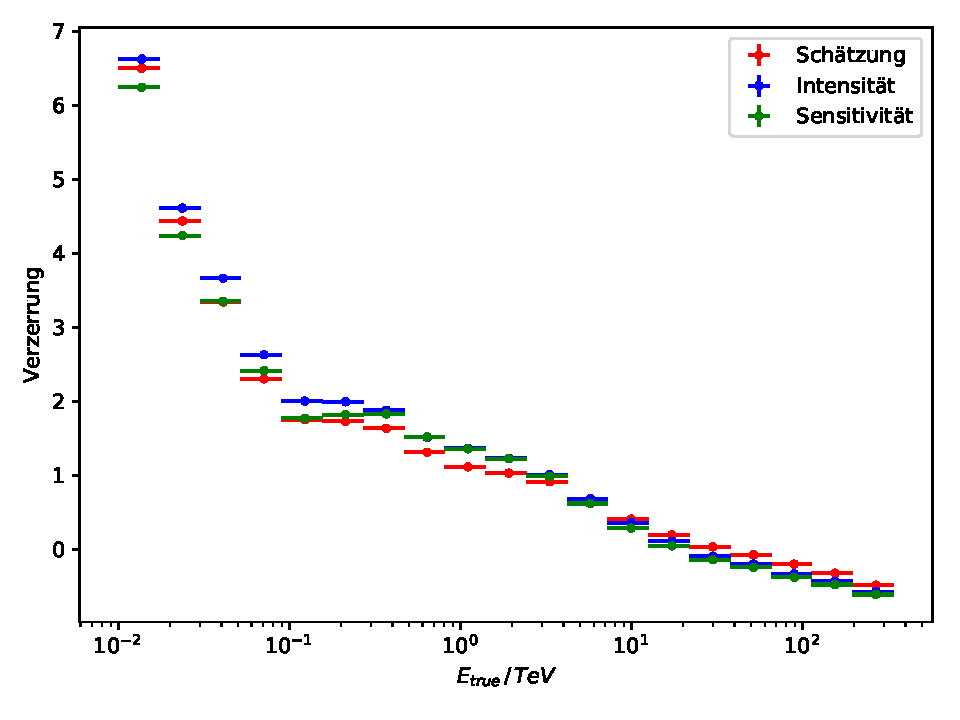
\includegraphics[width=0.7\textwidth]{Plots/RF_weights_bias.pdf}
  \centering
  \caption{Darstellung der Verzerrung für die arithmetische Mittelung, den Median und für eine gewichtete Mittelung mit der Intensität
            oder der Sensitivität als Gewicht.}
  \label{abb:w_bias}
\end{figure}
\begin{figure}
  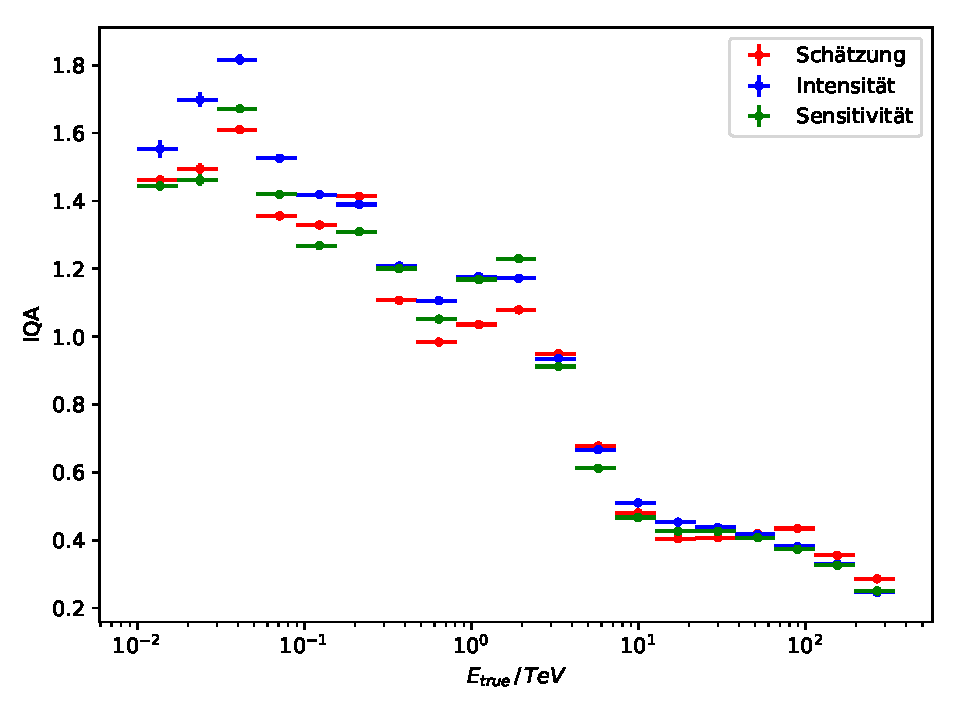
\includegraphics[width=0.7\textwidth]{Plots/RF_weights_resolution.pdf}
  \centering
  \caption{Auftragen des IQA des relativen Fehlers für verschiedene Energiebereiche, jeweils für den arithmetischen Mittelwert, den Median und
            für die mit der Intensität oder der Sensitivität gewichtet gemittelten Vorhersage.}
  \label{abb:w_IQA}
\end{figure}

Das Gewichten führt auf eine Energieschätzung, die in \autoref{abb:w_bias} und \autoref{abb:w_IQA} zu sehen ist.
Beide Gewichte führen nicht auf das gewünschte Ergebnis, wobei die Gewichtung mit der Intensität auf eine Verschlechterung der Performance führt.
Die Sensitivität scheint zwar ein Indikator für die Sichtbarkeit zu sein, jedoch scheint die Höhe der Gewichtung nicht ausreichend zu sein, um
die Fehlschätzungen ausreichend zu korrigieren.
Durch die Energieabhängigkeit der Intensität scheint dieses Attribut als Gewicht ungeeignet zu sein.
Jedoch verbessert sich der gemittelte quadratische Fehler auf $\SI{60.64}{\tera\eV\squared}$ im Vergleich zu der Gewichtung mit der Sensitivität, wo er bei
$\SI{66.05}{\tera\eV\squared}$ bleibt.

Das Ziel der Energieschätzung besteht darin die Energieauflösung der Teleskope zu verbessern, was jedoch nur durch eine Verringerung der
Verzerrung und des IQA gelingt und nicht durch die Verbesserung von Ergebnissen, die schon nahe an der Wahrheit liegen.
Daher führt eine gewichtete oder ungewichtete Mittelung über die Ergebnisse nicht zum Ziel.
Der Median sorgt für eine Verbesserung in niedrigen Energiebereichen, jedoch führt er zu einer Verschlechterung bei Energien von $(\num{0.1}-\num{1.0})\,\si{\tera\eV}$.
In diesem Bereich besitzt das CTA jedoch die größte Statistik, womit der Performancegewinn in Frage gestellt wird, was durch den
gleichbleibenden gemittelten quadratischen Fehler bestätigt wird.

%Einfacher Mittelwert über gleiches Event; Nutzung von unterschiedlichen Gewichten;

\section{Verschachtelung von Regressionsverfahren}
\label{sec:nest}

Schon die Wichtigkeit der eventspezifischen Attribute in \autoref{abb:first_FI} deutet darauf hin, dass die zusammengefassten Attributen eines Ereignisses
mehr Information beinhalten, als die teleskopspezifischen Attributen.
Daher wird nach der ersten Schätzung ein zweiter Random Forest trainiert, der mithilfe von eventspezifischen Attributen Schätzungen für jedes Ereignis abgibt.
Zu den Attributen gehören die Anzahl der ausgelösten Telskope, sowie SST, MST und LST, die totale Intensität, die arithmetisch gemittelte Schätzung des
ersten Waldes, die Mittelwerte und Standardabweichungen der skalierten Größen und die Mittelwerte, Standardabweichungen, Maximal- und Minimalwerte der
Schätzungen von den SST, MST und LST.
\begin{figure}
  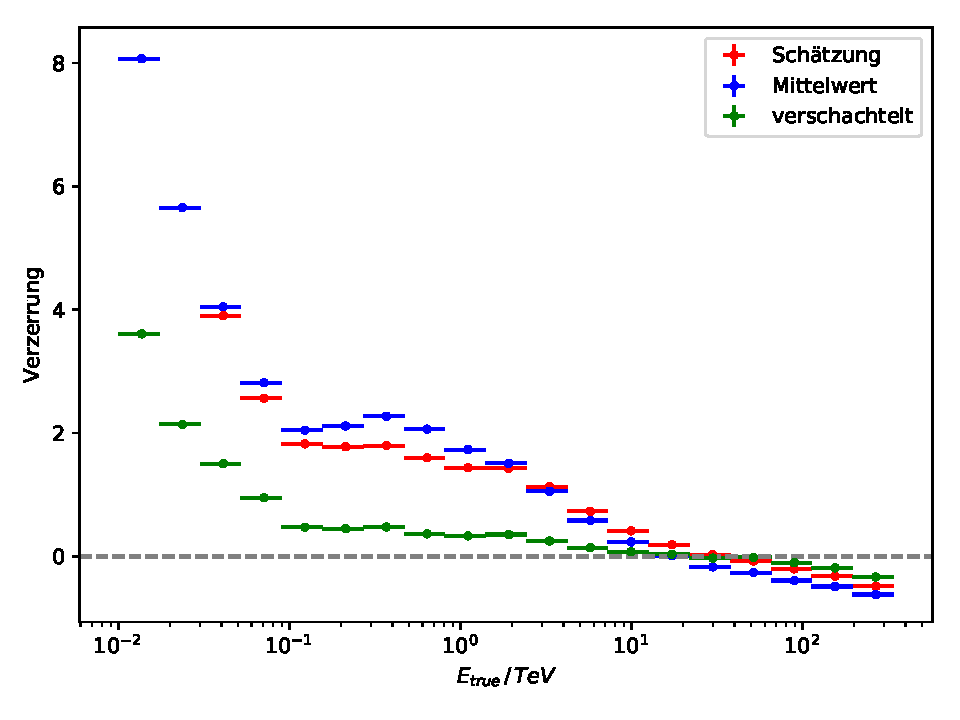
\includegraphics[width=0.7\textwidth]{Plots/RF_nested_bias.pdf}
  \centering
  \caption{Abbildung der Verzerrung nach einer Verschachtelung von zwei Random Forests. Es ist eine deutliche Verbesserung gegenüber der ersten Schätzungen
            zu erkennen.}
  \label{abb:nest_bias}
\end{figure}
\begin{figure}
  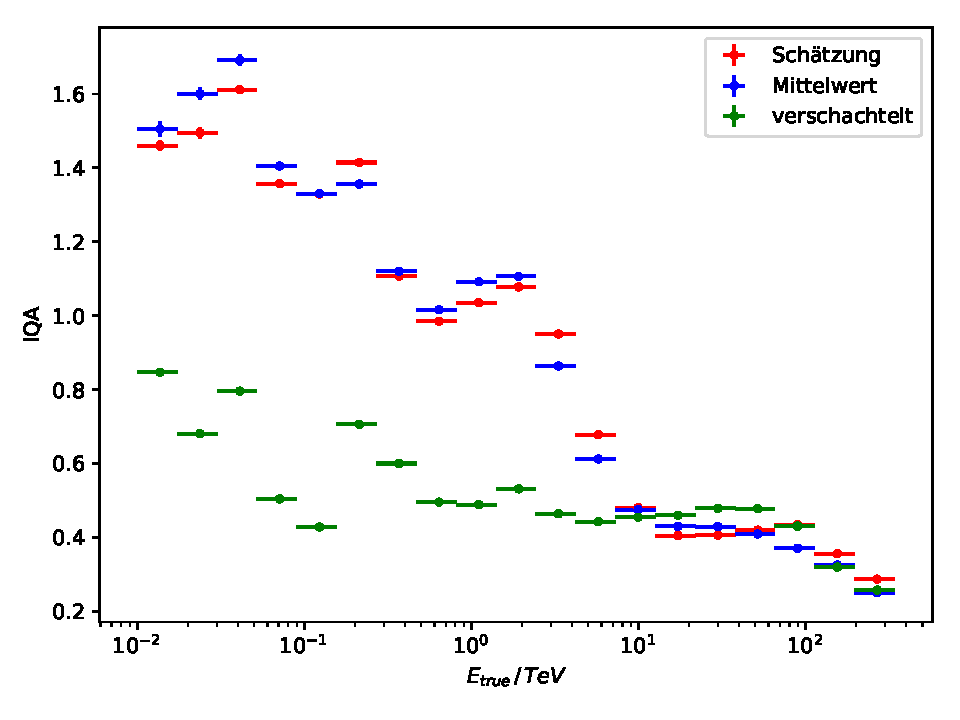
\includegraphics[width=0.7\textwidth]{Plots/RF_nested_resolution.pdf}
  \centering
  \caption{Abbildung des IQA für den zweiten Random Forest. Die Verschachtelung führt auf eine starke Verringerung des IQA bei niedrigen Energien.}
  \label{abb:nest_IQA}
\end{figure}

Der Random Forest wird mit $\num{498081}$ Ereignissen trainiert und mit genauso vielen getestet.
In \autoref{abb:nest_bias} und \autoref{abb:nest_IQA} ist die Performance des zweiten Schätzers dargestellt und der gemittelte quadrierte Fehler fällt
auf $\SI{37.74}{\tera\eV\squared}$.
Die Verschachtelung der Entscheidungswälder führt auf eine verbesserte Performance in allen Energiebereichen, sowohl bei der Verzerrung als auch bei dem IQA,
wodurch ein Übertraining durch den zweiten Wald ausgeschlossen werden kann.

Die genutzten Attribute haben eine starke Korrelation aufgrund der Gewinnung der Attribute aus der gleichen Information.
Dies ist durch die Anzahl an Ausreißer in \autoref{abb:second_FI} zu erkennen.
\begin{figure}
  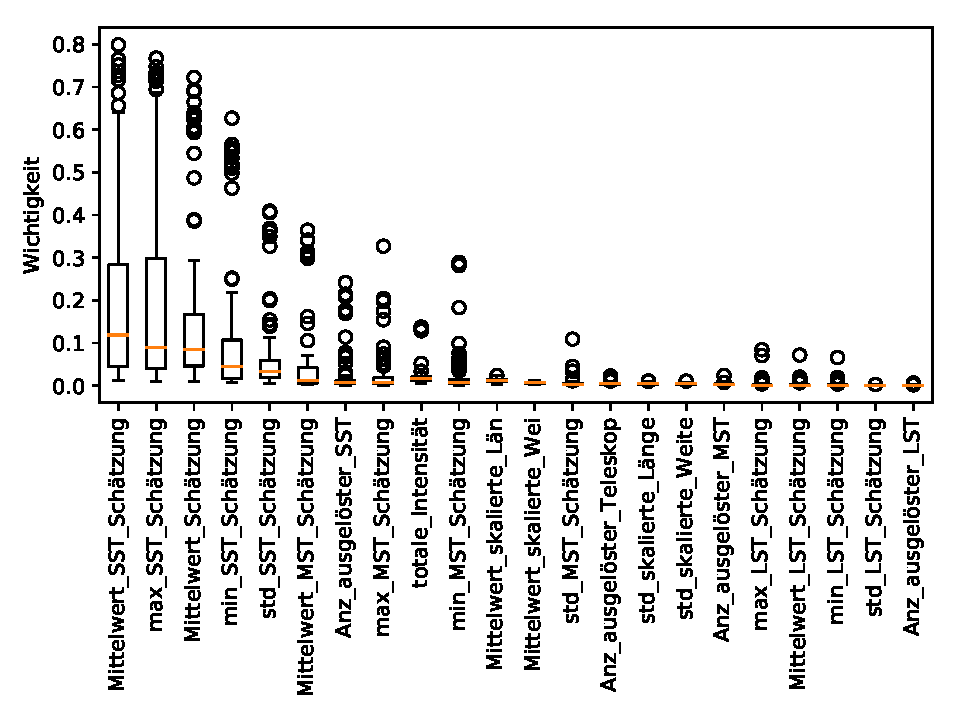
\includegraphics[width=0.7\textwidth]{Plots/feautureimportance_boxplot_secondForest.pdf}
  \centering
  \caption{Abbildung der Wichtigkeit der Attribute im zweiten Random Forest. Die Informationen der SST und die
          Schätzung des ersten Random Forest sind bedeutende Attribute und die hohe Fluktuation deutet auf eine
          Korreliertheit der Attribute hin.}
  \label{abb:second_FI}
\end{figure}
Eine genauere Untersuchung des Aufbaus der Entscheidungsbäume ergibt, dass die erste Seperation der Datensätze häufig mithilfe der gemittelten Schätzung geschieht,
um sich in den Unterbäumen auf die für diesen Energiebereich interessanten Attribute zu konzentrieren.
Die Anzahl der ausgelösten SST stellt zum Beispiel einen guten Parameter für hohe Energien dar, da solche Photonen große Schauer erzeugen, die
zu großen Cherenkov-Kegeln führen.
Eine geringe Anzahl an ausgelösten SST stellt jedoch kein Kriterium für eine geringe Photonenenergie dar, weil auch die Möglichkeit besteht, dass nur der
Rand des Schauers beobachtet wird.

Um die Frage zu beantworten, wie der Performancegewinn im Vergleich zum Zeitaufwand steht, wird zunächst die Komplexität für das Ausbauen des Entscheidungswaldes untersucht,
welche im Mittel bei
\begin{equation}
  \Theta (MK\tilde{N} \log^2\left(\tilde{N}\right))
\end{equation}
liegt\cite[96]{understanding_RF}.
Dies gilt für Random Forests mit $M$ Bäumen, die mit $K$ zufällig gezogenen Attributen und $N$ Datenpunkten vollständig ausgebaut werden.
Da das Bootstrapping in \textsc{scikit-learn} Datensätze erzeugt, die gleich groß wie der Originaldatensatz sind, gilt $\tilde{N}= N$.
Der Datensatz des zweite Entscheidungswald besitzt $N_2 \approx \frac{1}{5}N_1$ Datenpunkte, da im Mittel $\approx 5$ Teleskope auslösen.
Damit stellt
\begin{equation}
  \Theta \left(MK\frac{1}{5}\tilde{N_1} \log^2\left(\frac{1}{5}\tilde{N_1}\right)\right)
\end{equation}
den zusätzlichen Zeitauwand dar.
Da der Zeitaufwand der Schätzung, welcher
\begin{equation}
  \Theta\left(M\log\left(\frac{1}{5}N\right)\right)
\end{equation}
beträgt\cite[98]{understanding_RF}, für die angestrebte Echtzeitanalyse von größerem Interesse ist, steht der Performancegewinn noch besser da.
Außerdem werden die Entscheidungsbäume nicht vollständig ausgebaut, womit sich der Zeitaufwand deutlich verringert, jedoch können beide Entscheidungswälder nicht
parallelisiert werden, wodurch definitiv ein Zeitverlust ensteht.

\section{Transformation der Energie}

In \autoref{abb:Energie_RF} ist ein Abschneiden für niedrige Energien durch den Schätzer zu beobachten.
Durch die logarithmische Skala scheint es ein sehr drastischer Schnitt zu sein, jedoch ist der Fehler, der entsteht, wenn alle Energien $E_\gamma < \SI{0.1}{\tera\eV}$
auf $\SI{0.1}{\tera\eV}$ geschätzt werden, sehr gering.
Daher konzentriert sich der Algorithmus darauf die großen Energien richtig zu schätzen.
Dies führt jedoch auf einen großen relativen Fehler für kleine Energien, wie er in \autoref{abb:mean_median_bias} zu sehen ist und somit auf eine schlechte
Energieauflösung.

Eine bijektive Transformation auf $\symbb{R}^+$ mit
\begin{equation}
  E_{\symup{trafo}}=\ln(E_\gamma +3)
  \label{eqn:trafo}
\end{equation}
führt auf eine kleinere Zielmenge des Schätzers, wodurch die Performance weniger stark Energieabhängig ist.
Eine anschließende Rücktransformation mit
\begin{equation}
  E_\gamma = \exp \left(E_{\symup{trafo}}\right)-3
\end{equation}
führt wieder auf die richtige Energie.
\begin{figure}
  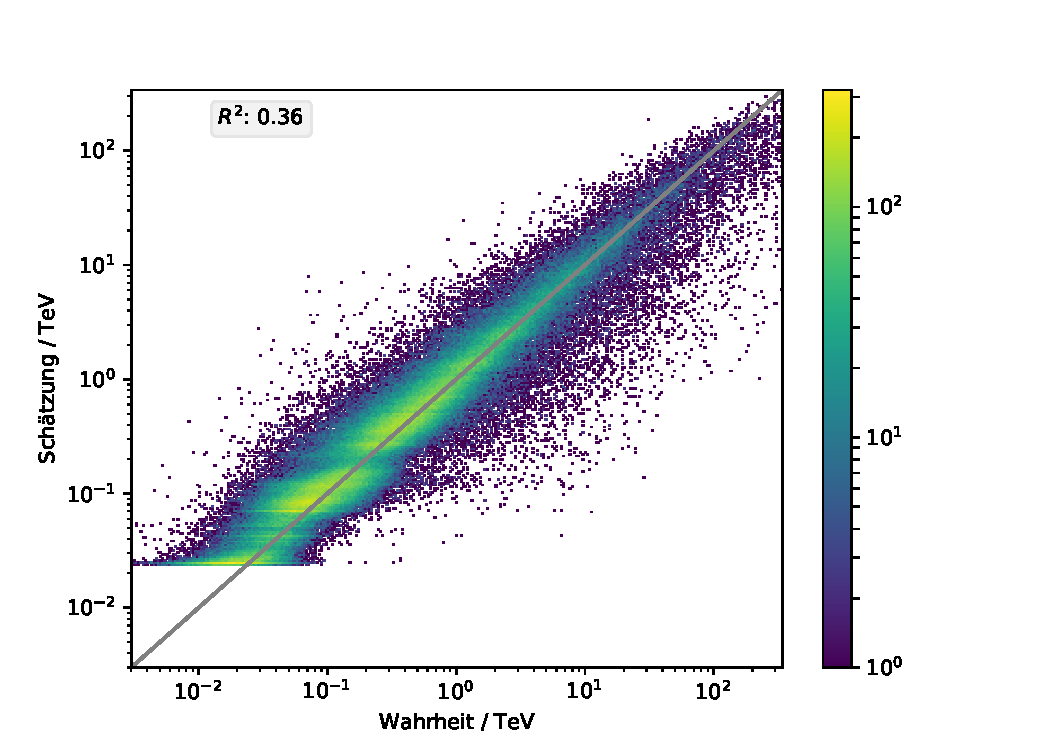
\includegraphics[width=0.7\textwidth]{Plots/trafo_encaps.pdf}
  \centering
  \caption{Abbildung der geschätzen Energie durch einen auf die transformierte Energie trainerten Random Forest. Der Schätzer schneidet fast eine Größenordnung
          später ab als der Schätzer aus \autoref{sec:first}.}
  \label{abb:Energie_trafo}
\end{figure}

Es wird das verschachtelte Modell aus \autoref{sec:nest} benutzt, wobei beide Schätzer auf die transformierte Energie trainiert werden.
\autoref{abb:Energie_trafo} zeigt, dass der Schätzer beinahe eine Größenordnung später abschneidet und die Transformation keinen Genauigkeitsverlust
in anderen Energiebereichen zufolge hat.
Der Schätzer scheint mehr Wert auf einen geringen Fehler bei kleinen Energien zu legen.
Schon das Verschachteln der Algorithmen sorgt für ein Herabsetzen der Grenze, da durch das frühe Trennen der Energiebereiche im Entscheidungsbaum, dem
Algorithmus die Möglichkeit gibt, sich auf die Verbesserung der geringen Energiebereiche zu konzentrieren.
Die Deutung von \autoref{abb:trafo_bias} und \autoref{abb:trafo_IQA} zeigt, dass die Transformation die Performance im Vergleich
zum Algorithmus aus \ref{sec:nest} verbessert.
\begin{figure}
  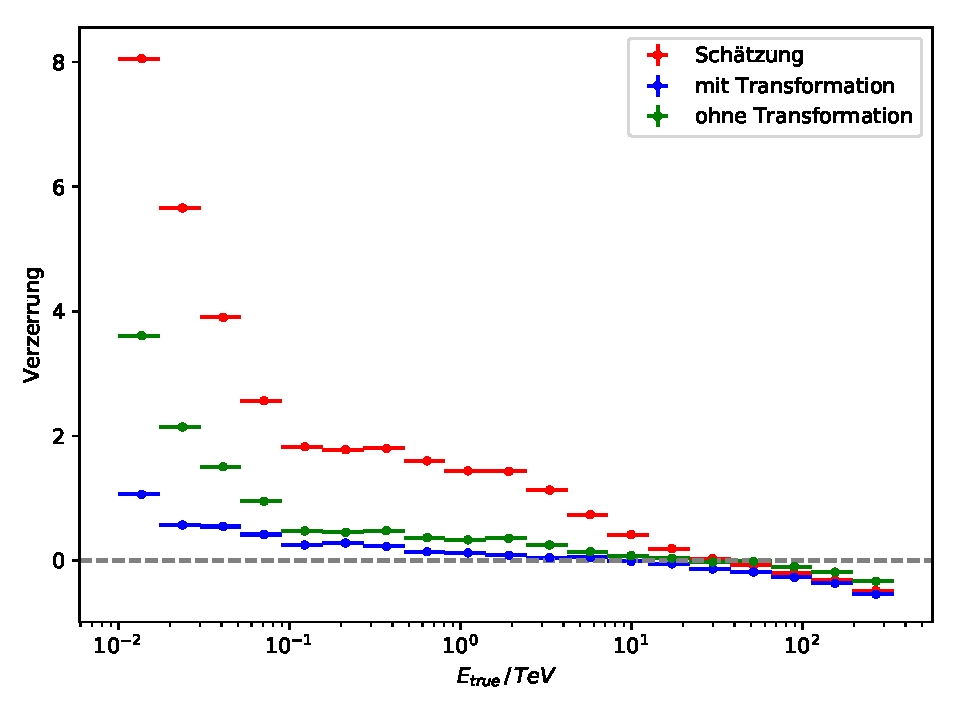
\includegraphics[width=0.7\textwidth]{Plots/trafo_nested_bias.pdf}
  \centering
  \caption{Darstellung der Verzerrung bei einer Schätzung mit und ohne Transformation der Art \eqref{eqn:trafo}. Die Transformation führt zu einer Verringerung
          des relativen Fehlers in geringen Energiebereichen.}
  \label{abb:trafo_bias}
\end{figure}
\begin{figure}
  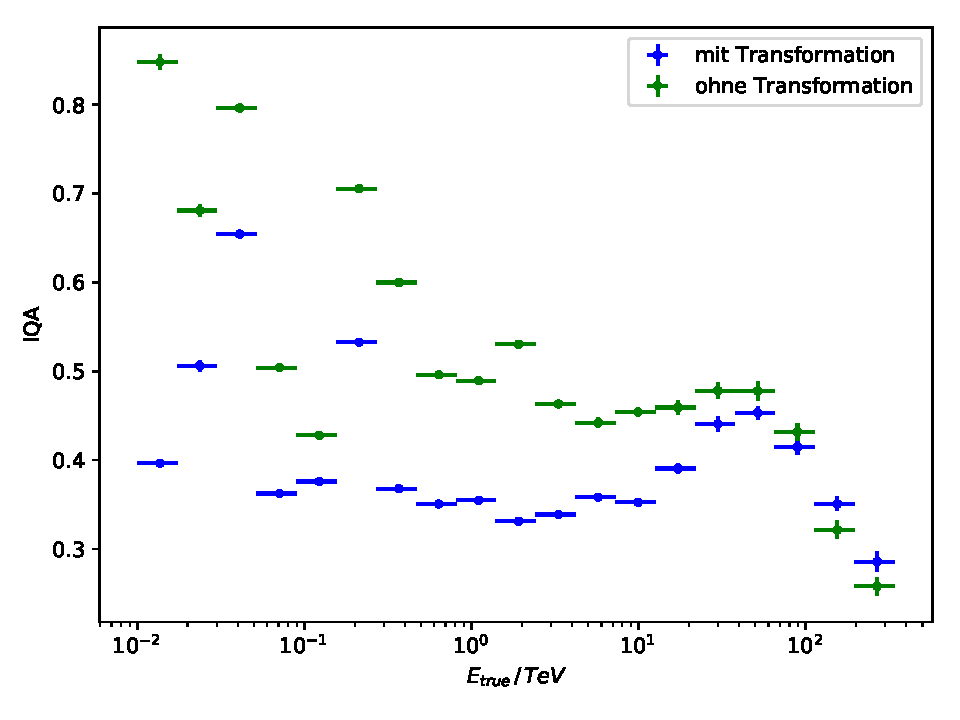
\includegraphics[width=0.7\textwidth]{Plots/trafo_nested_resolution.pdf}
  \centering
  \caption{Abbildung der Energieauflösung nach einer Transformation des Zielbereichs, welche auf eine Verbesserung in niedrigen Energiebereichen führt.}
  \label{abb:trafo_IQA}
\end{figure}
Sowohl der IQA als auch die Verzerrung des relativen Fehlers werden mithilfe der Transformation bei niedrigen Energien geringer.
Bei $E_\gamma > \SI{30}{\tera\eV}$ muss jedoch eine Verschlechterung der Verzerrung und Auflösung in Kauf genommen werden, welche jedoch eine große Verschlechterung
bezogen auf den absoluten Fehler bedeutet.

%mean squared error?
